\section{Graph}

\begin{frame}[fragile]{Graph}
  \begin{adjustbox}{max totalsize={.9\textwidth}{.7\textheight},center}
    \tikzstyle{every node}=[circle, draw, fill=black!50,
    inner sep=0pt, minimum width=4pt]
    % Tutte's 8-cage
    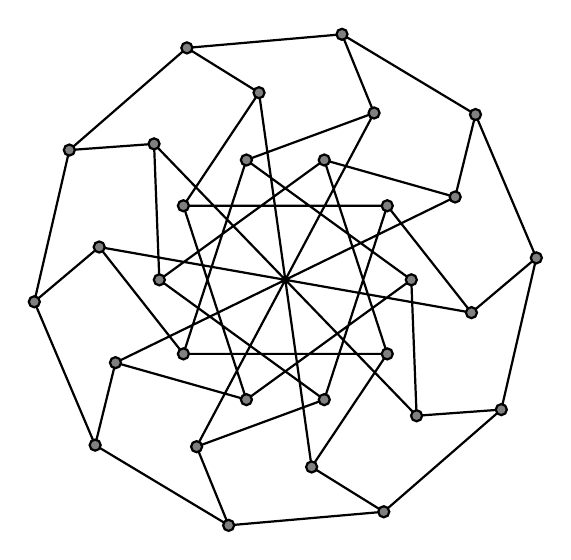
\begin{tikzpicture}[thick,scale=0.8]
      \draw \foreach \x in {0,36,...,324}
      {
        (\x:2) node {}  -- (\x+108:2)
        (\x-10:3) node {} -- (\x+5:4)
        (\x-10:3) -- (\x+36:2)
        (\x-10:3) --(\x+170:3)
        (\x+5:4) node {} -- (\x+41:4)
      };
    \end{tikzpicture}\quad

    % The largest 3-regular graph of diameter 3
    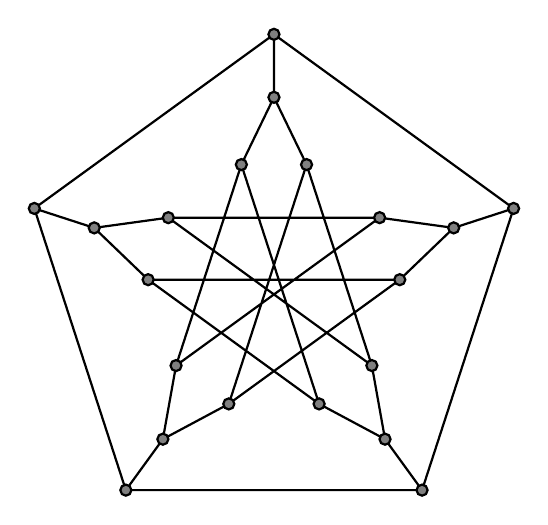
\begin{tikzpicture}[thick,scale=0.8]%
      \draw \foreach \x in {18,90,...,306} {
        (\x:4) node{} -- (\x+72:4)
        (\x:4) -- (\x:3) node{}
        (\x:3) -- (\x+15:2) node{}
        (\x:3) -- (\x-15:2) node{}
        (\x+15:2) -- (\x+144-15:2)
        (\x-15:2) -- (\x+144+15:2)
      };
    \end{tikzpicture}
  \end{adjustbox}
\end{frame}

\begin{frame}[fragile]{Content}
  \begin{easylist} \easyitem
    & 图的定义
    & 图的存储表示
    & 图的遍历
    & 图的连通性
  \end{easylist}
\end{frame}

\begin{frame}[fragile]
  \frametitle{图(Graph)}
  \begin{itemize}
  \item 图$G=(V, E)$, $V$是顶点(Vertex)集合,$E$是边/弧(Edge/Arc)的集合.
  \item 顶点的度、出度和入度
  \end{itemize}

  \begin{columns}[T]
    \column{0.5\textwidth}
    有向图:
    
    \begin{tikzpicture}[scale=1.0]
      \GraphInit[vstyle=Art]
      \Vertex{A}
      \Vertex[x=4,y=0]{B}
      \Vertex[x=0,y=2]{C}
      \Vertex[x=4,y=2]{D}
      \Edge[style={-Latex}](A)(D)

      \Edges[style={-Latex}](A,B,C, D)
      \Edges[style={-Latex}](A, C)
    \end{tikzpicture}
    
    \column{0.5\textwidth}
    无向图:
    
    \begin{tikzpicture}[scale=1.0]
      \GraphInit[vstyle=Art]
      \Vertex{A}
      \Vertex[x=4,y=0]{B}
      \Vertex[x=0,y=2]{C}
      \Vertex[x=4,y=2]{D}
      \Edge[style={}](A)(D)

      \Edges[style={}](A,B,C, D)
      \Edges[style={}](A, C)
    \end{tikzpicture}
  \end{columns}
\end{frame}

\begin{frame}[fragile]
  \frametitle{OK}
  \color{red}
  \begin{minted}[mathescape,
    linenos,
    numbersep=5pt,
    gobble=2,
    frame=lines,
    framesep=2mm]{java}
    class Test {
      
    }
  \end{minted}
\end{frame}

\begin{frame}[fragile]
  \frametitle{图的相关概念}
  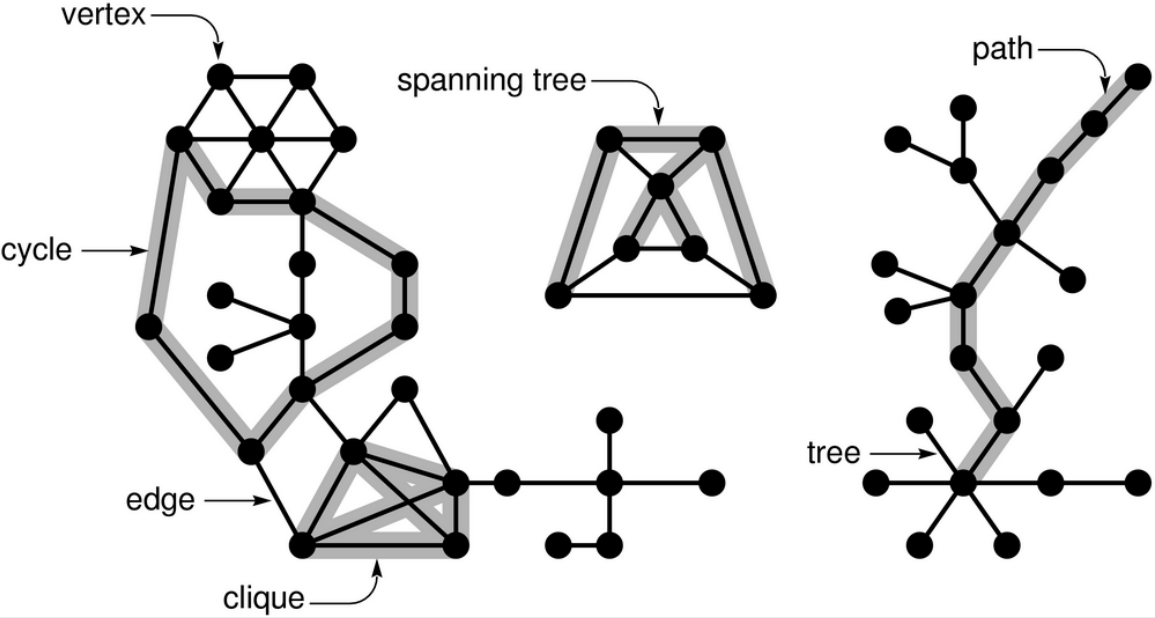
\includegraphics[width=0.9\textwidth]{figs/graph_concept.png}
\end{frame}

\begin{frame}[plain]
~  
\end{frame}

\begin{frame}[fragile]
  \frametitle{图的存储}
  如何表达下图的信息?
  \begin{columns}
    \column{0.4\textwidth}
    有向图:
    
    \begin{tikzpicture}[scale=1.3]
      \GraphInit[vstyle=Normal]
      \begin{scope}[rotate=180]
        \Vertices{circle}{$v_1$, $v_2$, $v_3$, $v_4$}
      \end{scope}
      \Edges[style={-Latex}]($v_1$,  $v_3$, $v_4$, $v_1$, $v_2$)
    \end{tikzpicture}
    
    \column{0.4\textwidth}
    无向图:
    
    \begin{tikzpicture}[scale=1.5]
      \GraphInit[vstyle=Normal]
      \begin{scope}[rotate=180]
        \Vertices{circle}{$v_1$, $v_2$, $v_3$, $v_4$}
      \end{scope}
      \Vertex{$v_5$}
      \Edges($v_1$, $v_2$, $v_3$, $v_4$, $v_1$)
      \Edges($v_2$, $v_5$, $v_3$)
    \end{tikzpicture}
  \end{columns}
  
  \pause
  \begin{itemize}
  \item 可用邻接矩阵表达顶点及其关系。
  \end{itemize}
\end{frame}


\begin{frame}[fragile]
  \frametitle{图的存储}
  \small
  \begin{columns}
    \column{0.4\textwidth}
    \begin{tikzpicture}[scale=1]
      \GraphInit[vstyle=Normal]
      \begin{scope}[rotate=180]
        \Vertices{circle}{$v_1$, $v_2$, $v_3$, $v_4$}
      \end{scope}
      \Edges[style={-Latex}]($v_1$,  $v_3$, $v_4$, $v_1$, $v_2$)
    \end{tikzpicture}
    \[
      \begin{blockarray}{ccccc}
         & v_1 & v_2 & v_3 & v_4 \\
        \begin{block}{c (c c c c)}
          v_1 & 0 & 1 & 1 & 0 \\
          v_2 & 0 & 0 & 0 & 0 \\
          v_3 & 0 & 0 & 0 & 1 \\
          v_4 & 1 & 0 & 0 & 0 \\
        \end{block}
      \end{blockarray}
    \]

    \column{0.4\textwidth}
    \begin{tikzpicture}[scale=1.0]
      \GraphInit[vstyle=Normal]
      \begin{scope}[rotate=180]
        \Vertices{circle}{$v_1$, $v_2$, $v_3$, $v_4$}
      \end{scope}
      \Vertex{$v_5$}
      \Edges($v_1$, $v_2$, $v_3$, $v_4$, $v_1$)
      \Edges($v_2$, $v_5$, $v_3$)
    \end{tikzpicture}

    \[
      \begin{blockarray}{cccccc}
         & v_1 & v_2 & v_3 & v_4 & v_5 \\
        \begin{block}{c (c c c c c)}
          v_1 & 0 & 1 & 0 & 1 & 0 \\
          v_2 & 1 & 0 & 1 & 0 & 1 \\
          v_3 & 0 & 1 & 0 & 1 & 1 \\
          v_4 & 1 & 0 & 1 & 0 & 0 \\
          v_5 & 0 & 1 & 1 & 0 & 0 \\
        \end{block}
      \end{blockarray}
    \]    
  \end{columns}
  
  \begin{itemize}
  \item 根据邻接矩阵,如何判断各顶点的度?
  \end{itemize}
\end{frame}
